\problem{}
\textbf{Given:} 
\begin{itemize}
    \item A graph $G = (V, E)$, which may be directed or undirected.
    \item Two distinguished vertices $s, t \in V$.
    \item A set of forbidden pairs $\mathcal{F} = \{(u_1, v_1), (u_2, v_2), \dots, (u_e, v_e)\} \subseteq V \times V$.
\end{itemize}


\noindent \textbf{Question:} 

Does there exist a path $P = (v_0, v_1, \dots, v_k)$ in $G$ from $s$ to $t$ such that:
\begin{enumerate}
    \item $v_0 = s$ and $v_k = t$.
    \item For each forbidden pair $(u_i, v_i) \in \mathcal{F}$, the path $P$ contains at most one of $u_i$ or $v_i$.
\end{enumerate}

\noindent Prove that this problem is NP-complete.

\noindent \textbf{Hint:} see the gadgets below.

\begin{figure}[h]
    \centering
    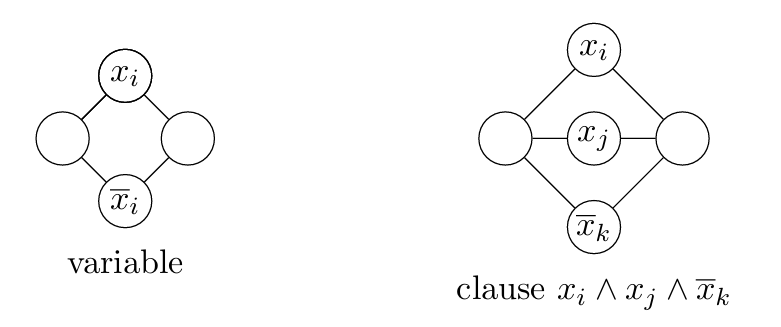
\includegraphics[width=0.7\textwidth]{gadget_example.png}
    \label{fig:gadget}
\end{figure}

\noindent \textbf{Proof:}

\noindent\textbf{Step 1: the Forbidden-Pair Constrained Path problem \( \in \mathrm{NP}\).} \\

Given a candidate path $P$, we can verify in polynomial time:
\begin{enumerate}
    \item Check $P$ starts at $s$ and ends at $t$
    \item Check $P$ is a valid path in $G$ (adjacent vertices connected by edges)
    \item For each forbidden pair $(u, v) \in \mathcal{F}$, check $P$ contains at most one of $u$ or $v$
\end{enumerate}
All checks take $O(|V| + |E| + |\mathcal{F}|)$ time. Thus, the problem is in NP.

\noindent\textbf{Step 2: Reduction from \textsc{3SAT } to the Forbidden-Pair Constrained Path problem.} \\

We choose \textbf{3SAT} as our NP-complete problem $B$.

Let $\phi$ be a 3SAT formula with $n$ variables $x_1, \dots, x_n$ and $m$ clauses $C_1, \dots, C_m$.

We construct an instance of the Forbidden-Pair Constrained Path problem:

\textbf{Graph Construction}

Vertices:
\begin{itemize}
    \item Start vertex $s$, terminal vertex $t$
    \item For each variable $x_i$: vertices $X_i$ (true) and $\overline{X}_i$ (false)
    \item For each clause $C_j$ and each literal $\ell_{jr}$ ($r = 1,2,3$): vertex $C_{jr}$
\end{itemize}

Edges:
\begin{itemize}
    \item $s \to X_1$, $s \to \overline{X}_1$
    \item For $i = 1$ to $n-1$: $X_i \to X_{i+1}$, $X_i \to \overline{X}_{i+1}$, $\overline{X}_i \to X_{i+1}$, $\overline{X}_i \to \overline{X}_{i+1}$
    \item $X_n \to C_{jr}$ for all $j, r$; $\overline{X}_n \to C_{jr}$ for all $j, r$
    \item $C_{jr} \to t$ for all $j, r$
\end{itemize}

\textbf{Forbidden Pairs Construction}
\begin{enumerate}
    \item \text{Variable consistency:} For each $i$, $(X_i, \overline{X}_i)$
    \item \text{Clause satisfaction:} For each clause $C_j$: $(C_{j1}, C_{j2})$, $(C_{j2}, C_{j3})$, $(C_{j3}, C_{j1})$
    \item \text{Literal enforcement:} For each $C_{jr}$, if $\ell_{jr} = x_k$, then $(C_{jr}, \overline{X}_k)$; if $\ell_{jr} = \overline{x}_k$, then $(C_{jr}, X_k)$
\end{enumerate}

\noindent\textbf{Step 3: Correctness (equivalence).} \\

\textbf{($\Rightarrow$) If $\phi$ is satisfiable, then path exists}

Let $A$ be a satisfying assignment for $\phi$. Construct path $P$ as follows:
\begin{enumerate}
    \item Start at $s$
    \item For each variable $x_i$: if $A(x_i) = \text{true}$, go to $X_i$; else go to $\overline{X}_i$
    \item For each clause $C_j$: choose a literal $\ell_{jr}$ that is true under $A$, go to $C_{jr}$
    \item Go to $t$
\end{enumerate}

Verification:
\begin{itemize}
    \item Variable consistency: Path contains exactly one of $X_i$ or $\overline{X}_i$ for each $i$
    \item Clause constraints: At most one $C_{jr}$ per clause due to forbidden pairs $(C_{j1}, C_{j2})$, etc.
    \item Literal enforcement: If $C_{jr}$ is visited, then $\ell_{jr}$ is true, so the opposite literal vertex is not in path
\end{itemize}

\textbf{($\Leftarrow$) If path exists, then $\phi$ is satisfiable}
Given a valid path $P$:
\begin{enumerate}
    \item Extract variable assignment: If $X_i \in P$, set $x_i = \text{true}$; if $\overline{X}_i \in P$, set $x_i = \text{false}$
    \item For each clause $C_j$, exactly one $C_{jr}$ is in $P$ (due to forbidden pairs)
    \item Since $(C_{jr}, O_{jr})$ is forbidden (where $O_{jr}$ is opposite literal vertex), $O_{jr} \notin P$
    \item Thus, the literal $\ell_{jr}$ must be true under the assignment
    \item Therefore, all clauses are satisfied
\end{enumerate}


The reduction constructs:
\begin{itemize}
    \item $O(n + m)$ vertices
    \item $O(n + nm)$ edges
    \item $O(n + m)$ forbidden pairs
\end{itemize}
All steps are polynomial in the size of the 3SAT instance.

Therefore, the Forbidden-Pair Constrained Path problem is \textbf{NP-complete}.
\newpage